\chapter{アンダー・サンプリング}
    \section{アンダー・サンプリングされた信号の DTFT}
        \label{アンダー・サンプリングされた信号の DTFT}
        \subsection{主張}
            記号を次のように定義する。
            \begin{itemize}
                \item $R\in\naturalNumbers,\;R\geq 2$ : アンダー・サンプリング・レート
                \item $\xd:\integers\to\complexNumbers$ : 離散時間信号
                \item $\Ts>0$ : $\xd$ のサンプル周期
                \item $\yd$ : $\xd$ を $1/R$ にアンダー・サンプリングした離散時間信号。つまり $\yd(n) = \xd(nR)$ 。
                \item $\Xd$ : $\xd$ のDTFT
                \item $\Yd$ : $\yd$ のDTFT
            \end{itemize}
            このとき $\Yd$ は次式で表される。
            \[ \Yd(\omega) = \frac{1}{R}\sum_{n=0}^{R-1} \Xd\parens*{\omega-n\frac{2\pi}{R\Ts}} \]
            $\Yd$ は $\omega$ に関する $2\pi/(R\Ts)$ 周期関数となり、$\Yd$ の第1 Nyquist 領域は $S_{\text{N},Y} \coloneq [-\pi/(R\Ts),-\pi/(R\Ts))$ となる。
            \par
            全体に $1/R$ が掛けられているが、振幅が $1/R$ になるわけではない。
            DTFT の内積計算の対象となる点の数が $1/R$ に減ったことに起因する。
            \par
            $\Xd$ の台のうち $\xd$ の第1 Nyquist 領域 $S_{\text{N},X} \coloneq [-\pi/\Ts, \pi/\Ts)$ にある部分を $S_X$ とする。
            エイリアシングが生じない必要十分条件は $S_X\subset S_{\text{N},X}$ である。
            ここで言うエイリアシングとは、$S_X$ を $2\pi/(R\Ts)$ の整数倍ずつ平行移動しながら無限に複製したものを考えたとき、複製された $S_X$ 同士に重なりが生じることを指す。
        \subsection{導出}
            \begin{align}
                \Yd(\omega) &= \sum_{n=-\infty}^\infty \yd(n)\exp(-i\omega nR\Ts) = \sum_{n=-\infty}^\infty \xd(nR)\exp(-i\omega nR\Ts) \nonumber \\
                &= \sum_{m=-\infty}^\infty u(m)\xd(m)\exp(-i\omega m\Ts) \quad \text{where} \quad u(m) \coloneq \begin{cases}
                    1 & (m\in R\integers) \\
                    0 & (\text{otherwise})
                \end{cases} \nonumber  \\
                &= \DTFTwithArg{u\xd}{\omega} \nonumber \\
                &= \frac{\Ts}{2\pi}\integrate{-\pi/\Ts}{\pi/\Ts}{\Xd(\omega-\tilde{\omega})U(\tilde{\omega})}{}{\tilde{\omega}} \quad \text{where} \quad U(\omega) \coloneq \frac{2\pi}{R\Ts}\sum_{m=-\infty}^\infty\delta\parens*{\omega - n\frac{2\pi}{R\Ts}} \nonumber \\
                &= \frac{1}{R} \integrate{-\pi/\Ts}{\pi/\Ts}{\Xd(\omega-\tilde{\omega})\sum_{n=-\infty}^{\infty}\delta\parens*{\tilde{\omega}-n\frac{2\pi}{R\Ts}}}{}{\tilde{\omega}} \label{equation:アンダー・サンプリングされた信号の周波数スペクトラム 1}
            \end{align}
            被積分関数の $\Xd$ とデルタ関数列を次の図に示す。
            \begin{figure}[H]
                \centering
                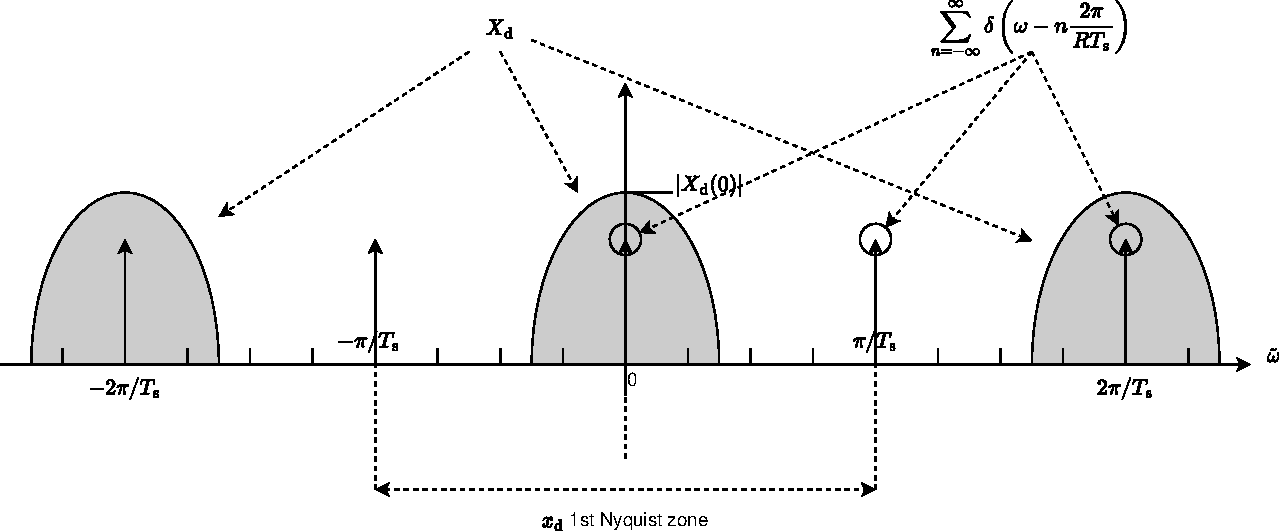
\includegraphics[keepaspectratio, scale=0.7]
                {\currfiledir/figs/X_d_and_delta_impulse_series.pdf}
                \caption{$\Xd$ とデルタ関数列($R=2$)}
            \end{figure}
            $\Xd$ が $2\pi/\Ts$ 周期関数であること、\cref{equation:アンダー・サンプリングされた信号の周波数スペクトラム 1} の積分範囲が $[-\pi/\Ts,\pi/\Ts]$ であること、および $R$ が偶数の場合に積分範囲の両端点で生じる、デルタ関数の中心から左右半分と $\Xd$ との積の積分を考慮すると、\cref{equation:アンダー・サンプリングされた信号の周波数スペクトラム 1} は次式と等しいことが解る。
            \begin{align}
                \Yd(\omega) &= \frac{1}{R}\sum_{n=-\floor{R/2}}^{\floor{R/2}} \integrate{-\pi/\Ts}{\pi/\Ts}{\Xd(\omega-\tilde{\omega})\delta\parens*{\tilde{\omega}-n\frac{2\pi}{R\Ts}}}{}{\tilde{\omega}} \nonumber \\
                &= \frac{1}{R}\sum_{n=0}^{R-1} \Xd\parens*{\omega-n\frac{2\pi}{R\Ts}} \label{equation:アンダー・サンプリングされた信号の周波数スペクトラム 2}
            \end{align}
            また同時に、$\Yd$ が $\omega$ に関する $2\pi/(R\Ts)$ 周期関数であることも解る。
            \par
            エイリアシングが生じないことと $S_X \subset S_{N,\text{X}}$ が同値であることが解る。
            $\Yd$ を次の図に示す。
            \begin{figure}[H]
                \centering
                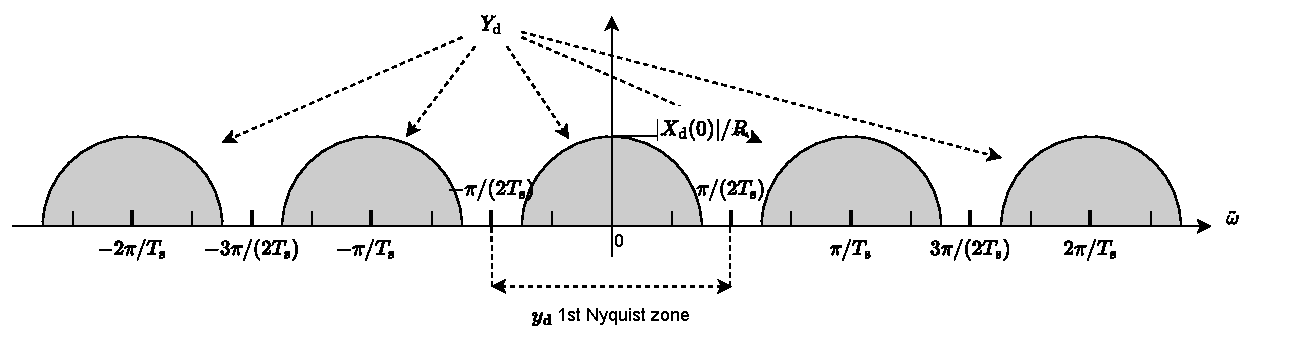
\includegraphics[keepaspectratio, scale=0.7]
                {\currfiledir/figs/Yd.pdf}
                \caption{$\Yd$}
            \end{figure}
        \subsection{正規化角周波数で比較する}
            フィルタ設計に於いてはしばしばダウン・サンプリング後の第1 Nyquist 領域に関心がある、すなわち横軸が正規化角周波数で表されたスペクトラムに関心がある。
            この場合は $\Yd$ のグラフの見た目が異なる。
            正規化角周波数で表示すると次式となる。
            \[ \tilde{\Yd}(\Omega) \coloneq \Yd(\Omega/(R\Ts)) \]
            正規化角周波数で表示されたグラフでは、アンダー・サンプリングされた信号のスペクトラムは元の信号のスペクトラムを \cref{equation:アンダー・サンプリングされた信号の周波数スペクトラム 2} に従って複製して並べた後、横軸方向に $R$ に拡大した形になる。
        \subsection{数値例}
            いくつかの数値例が下記の Mathematica ノートブックにある。
            下記の $x$ はサンプリング前の連続時間信号である。
            \begin{itemize}
                \item \verb|DTFT_of_under-sampled_signal.nb|: $x(t) = A\exp(-t^2/(2\sigma^2))$
                \item \verb|DTFT_of_under-sampled_signal_example2.nb|: $x(t) = e^{-12.5 t^2}\cos(10\pi t)$
            \end{itemize}
